\chapterimage{Mavrica.jpg} % Chapter heading image

\chapter{Detektorji svetlobe}

Za konec bomo spoznali še detektorje svetlobe, ki so nepogrešljivi
pri kvantitativni obravnavi optičnih pojavov. Detektorji se med seboj razlikujejo
po svojih specifikacijah, ki jih bomo opisali v nadaljevanju, in po načinu delovanja. 
Nazadnje bomo spoznali šum, ki omejuje uporabnost naprav.

\section{Osnovne karakteristike detektorjev}

Osnovna naloga optičnih detektorjev je pretvoriti vpadni svetlobni signal 
v nek drug signal, ki ga lahko natančno merimo. Navadno sta to električni tok 
ali električna napetost, ki sta sorazmerna z močjo vpadne svetlobe 
(in ne z amplitudo električne poljske jakosti). V grobem delimo detektorje v dve skupini, 
na termične in kvantne. Prvi pretvorijo energijo vpadne svetlobe 
v toploto, drugi pa temeljijo na fotoefektu, kjer vpadli foton izbije elektron ali 
ustvari par elektron-vrzel.

Pri termičnih detektorjih zaznamo svetlobo tako,
da merimo povečanje temperature senzorja zaradi absorbirane svetlobe in taki detektorji
zaznavajo energijo vpadle svetlobe. Njihov odziv je razmeroma počasen, zato jih uporabljamo
predvsem za merjenje optične moči, lahko tudi zelo velike. Po drugi strani pa je odziv
termičnih detektorjev neodvisen
od valovne dolžine vpadne svetlobe, zaradi česar so termični detektorji uporabni na 
širokem območju od globoke ultravijolične do daljne infrardeče svetlobe. Uporaba
prevlada predvsem v infrardrečem, teraherčnem ali celo mikrovalovnem območju, kjer so 
drugi detektorji bistveno manj občutljivi. 
Primeri termičnih detektorjev so bolometer, termočlen in piroelektrični detektor.

Druga skupina so kvantni detektorji, v katerih se
fotoni absorbirajo in povzročijo pojav prostih nosilcev naboja. Taki detektorji
torej zaznavajo število vpadlih fotonov. Odlikuje jih zelo hiter odziv (tipično pod $\si{\micro\second}$)
in velika občutljivost. Njihova slabost je omejen obseg valovnih dolžin,
pri katerih zaznavajo svetlobo, poleg tega jih je za optimalno delovanje treba 
hladiti. Primeri so vakuumske, polprevodniške in plazovne fotodiode.
\begin{figure}[h]
\centering
\def\svgwidth{65truemm} 
\input{slike/11_ShemaTermKv.pdf_tex}
\caption{Primerjava spektralnega odziva termičnega in kvantnega detektorja}
\label{fig:shemaTermKv}
\end{figure}

Osnovne karakteristike, ki omogočajo primerjavo med detektorji in določajo njihovo uporabnost,
so občutljivost, spektralni odziv, odzivni čas in prag detekcije. 

\begin{enumerate}
\item Občutljivost detektorja $R$ pove, koliko signala dobimo na enoto vpadnega svetlobnega toka. 
Enota za občutljivost je tako A/W ali V/W. 
\item Spektralni odziv pove, kako se občutljivost spreminja z valovno dolžino $R(\lambda)$.
Pri termičnih detektorjih je $R(\lambda)$ konstanta, medtem ko kvantni detektorji 
delujejo le v določenem območju valovnih dolžin, ki je odvisen od snovi, 
iz katere je detektor narejen. 
\item Odzivni čas pove, kako hitro se detektor odzove na spremembo optičnega signala. 
\item Prag detekcije pove, pri kolikšni vpadni svetlobni moči postane razmerje med signalom ($S$)
in šumom ($N$, {\it noise}) enako $S/N = 1$. 
\end{enumerate}

\section{Termični detektorji}
Termične detektorje se zaradi njihovega razmeroma počasnega odziva uporablja predvsem 
za merjenje vpadne moči in za detekcijo svetlobe tistih valovnih dolžin, za katere 
ni drugih preprostih ali učinkovitih detektorjev. Pogosto se uporabljajo za termografske 
kamere in v astronomiji.

Delovanje termičnih detektorjev temelji na spremembi temperature zaradi absorpcije svetlobe 
(energije), detektorji pa se med seboj razlikujejo predvsem v načinu pretvorbe spremembe 
temperature v električni signal.
Tipalo termičnih detektorjev mora biti pri vseh vrstah dobro počrnjeno, da absorbira
svetlobo v čim širšem spektralnem območju. Čeprav je njihova občutljivost načeloma 
neodvisna od valovne dolžine vpadne svetlobe, se v praksi pojavijo omejitve zaradi
prepustnosti okna in absorpcijskega spektra črnega nanosa. Tipala so majhna, zato 
da dosežemo čim hitrejši odziv, ki pa je kljub temu navadno počasnejši od 1~ms. Sodobnejši
detektorji se po odzivnem času že približujejo kvantnim, saj dosegajo odzivne čase tudi do
$\sim 10~\si{\micro\second}$. Termične detektorje uporabljamo pri sobni temperaturi, 
za zahtevne meritve pa jih hladimo na nekaj K. 

Obravnavajmo termični detektor, katerega tipalo naj ima toplotno kapaciteto $C$. Toplota
se s tipala odvaja v nek toplotni rezervoar s temperaturo $T_0$, 
toplotne izgube pa označimo z $\Lambda$. Ko na tipalo vpada svetloba moč $P$, začne
temperatura tipala $T$ zaradi absorpcije svetlobe naraščati, hkrati pa se tipalo 
ohlaja zaradi odtekanja toplote:
\beq
\frac{dW}{dt} = C \frac{dT}{dt} = P - \Lambda (T-T_0).
\label{TD1}
\eeq
V stacionarnem stanju, ki ga dosežemo pri konstantnem vpadnem svetlobnem toku, se
temperatura tipala ne spreminja in razlika temperature tipala in rezervoarja je 
\beq
T - T_0 = \frac{P}{\Lambda}.
\label{temp_sens}
\eeq
Občutljivost detektorja, ki je sorazmerna z razliko temperatur, 
je torej obratno sorazmerna z močjo, s katero se tipalo hladi. Za večjo občutljivost moramo
torej toplotne izgube detektorja kar se da zmanjšati. 

Po enačbi~(\ref{TD1}) se temperatura približuje stacionarni vrednosti s časovno konstanto 
\beq
\tau = \frac{C}{\Lambda},
\label{TermD_t}
\eeq
ki je ključni parameter za določanje odzivnega časa detektorja. Odzivni
čas je sorazmeren s kapaciteto senzorja, zato so tipala praviloma zelo majhna.
Vidimo, da moramo za dosego čim krajšega odzivnega časa toplotne izgube kar se da povečati. Če velike
izgube skrajšajo odzivni čas, pa po drugi strani zmanjšajo občutljivost (enačba~\ref{temp_sens}), 
zato pri termičnih detektorjih ne moremo imeti hkrati velikega in hitrega odziva. 
Če želimo toplotne izgube povečati, da s tem skrajšamo odzivni čas, detektorje hladimo z zrakom 
ali celo z vodo, majhne toplotne izgube pa so omejene s sevanjem.  

Podrobneje poglejmo odziv termičnega detektorja od vpadne moči. Naj se vpadna moč
spreminja s časom, temperatura na detektorju pa temu sledi z določeno zakasnitvijo. Odziv
najlepše izračunamo v Fourierevem prostoru. Vpadno moč in temperaturo izrazimo kot
\beq
P(t) = \int_{-\infty}^{\infty} P_\omega e^{i\omega t}d\omega \quad \mathrm{in} \quad
T = T_0 + \int_{-\infty}^{\infty} T_\omega e^{i\omega t}d\omega.
\label{TermTF}
\eeq
To vstavimo v enačbo~(\ref{TD1}) in dobimo
\beq
\int_{-\infty}^{\infty} i \omega T_\omega e^{i\omega t}d\omega = \frac{1}{C}
\int_{-\infty}^{\infty} (P_\omega - \Lambda T_\omega) e^{i\omega t}d\omega.
\eeq
Enačbi zadostimo, če izenačimo člene pred vsako spektralno komponento posebej
\beq
i \omega T_\omega = \frac{1}{C}\left(P_\omega - \Lambda T_\omega\right).
\eeq
Če vpeljemo odzivni čas $\tau$ (enačba~\ref{TermD_t}), sledi
\beq
T_\omega = \frac{1}{\Lambda}\left(\frac{1}{1+i \omega \tau}\right)P_\omega.
\label{TermOdziv}
\eeq

\begin{definition}
Pokaži, da je odziv termičnega detektorja na zelo kratek svetlobni sunek oblike 
$P(t) = P_0 \delta(t-t_0)$ enak 
\beq
T(t)=\frac{iP_0}{\Lambda}e^{-(t-t_0)/\tau}.
\eeq
\end{definition}

\subsection*{Bolometer}
Bolometer je termični detektor, pri katerem zaznavamo spremembo električne upornosti
zaradi spremembe temperature tipala\footnote{Prvi bolometer je leta 1881 naredil
ameriški fizik, astronom in letalski inženir Samuel Pierpont Langley, 1834--1906.}. 
Tipalo je praviloma počrnjena tanka ploščica, 
navadno je narejena iz termistorja, polprevodnika ali superprevodnika. Tipalo preko
referenčnega upora priključimo na napetost, preko kondenzatorja pa merimo napetost na njem.
Za meritve konstantega svetlobnega toka tipalo navadno vežemo v Wheatstonov mostiček. V obeh
primerih za referenčni upor vzamemo kar enako tipalo, ki ga zaščitimo pred vpadno svetlobo, 
tako da postane sistem neobčutljiv na morebitne spremembe temperature okolice.
\begin{figure}[h!]
\centering
\def\svgwidth{90truemm} 
\input{slike/11_bolometer.pdf_tex}
\caption{Shema bolometra}
\label{fig:Bolometer-shema}
\end{figure}

Prednost bolometrov bolometrih s termistorjem je približno linearna zveza med upornostjo in 
temperaturo. Uporabljamo jih predvsem za merjenje večjih vpadnih moči, saj taki 
detektorji niso zelo občutljivi ($R\sim 100~\si{\volt/\watt}$). 
So pa robustni, stabilni in delujejo pri sobni 
temperaturi. Odzivni časi so okoli $\tau \sim 1-20~\si{\milli\second}$. 
Pri polprevodniških bolometrih upornost narašča eksponentno s temperaturo. 
Primerni so za detekcijo teraherčnih valovanj, vendar mora biti za ta namen 
bolometer (npr. germanijev) hlajen s tekočim helijem. Tako lahko dosežemo
občutljivosti večje od $R \sim 10^8~\si{\volt/\watt}$. Zelo občutljivi so tudi 
detektorji s superprevodnimi tipali, saj je odvisnost upornosti od temperature v bližini
prehoda v superprevodno stanje zelo velika ($R \sim 10^3~\si{\volt/\watt}$).

\begin{figure}[h]
\centering
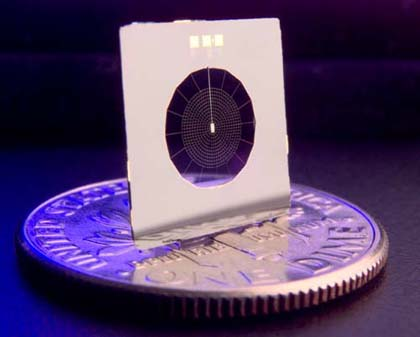
\includegraphics[width=80truemm]{slike/11_Bolometer.jpg}
\caption{Bolometer za merjenje prasevanja. Premer kovanca za primerjavo je 18~mm. 
Vir: NASA/JPL-Caltech.}
\label{fig:Bolometer}
\end{figure}

\subsection*{Termočlen}
Termočlen je sestavljen iz dveh različnih vodnikov. En spoj vodnikov počrnimo, drugega, 
referenčnega, pa zaščitimo pred svetlobo. Zaradi vpadne svetlobe se počrnjeni spoj 
segreje, med obema spojema nastane temperaturna razlika in zaradi termoelektričnega 
pojava tudi električna napetost, ki jo lahko merimo. Pri tem pazimo, da je prevodnost
vodnikov čim večja, toplotna prevodnost pa čim manjša. Odzivni čas termočlenov je 
okoli $\tau \sim 10-20~\si{\milli\second}$, občutljivost pa okoli $R \sim 10~\si{\volt/\watt}$.
Ker so napetosti, ki se pojavijo med stikoma, razmeroma majhne (le okoli 
$\sim 10~\si{\micro\volt/K}$) pogosto vežemo več termočlenov zaporedno v termobaterijo, navadno
nekaj deset. Občutljivost s tem naraste na $R \sim 200~\si{\volt/\watt}$, podaljša 
pa se časovna konstanta $\tau \sim 10-2000~\si{\milli\second}$.

\subsection*{Piroelektrični detektor}
Piroelektriki so snovi brez centra inverzije, v katerih je lastna električna 
polarizacija odvisna od temperature (npr. LiTaO$_3$, triglicin sulfat TGS,
polivinilidenfluorid PVDF in vsi feroelektriki). Piroelektrični detektor je narejen iz 
ploščice piroelektrične snovi med dvema elektrodama oziroma ploščama kondenzatorja.
Ko se ploščica zaradi absorbirane svetlobe segreje, se ji spremeni polarizacija in 
med elektrodama se pojavi premikalni tok, ki ga merimo na merilnem uporniku.

Zveza med spremembo temperature in spremembo polarizacije je
\beq
dP = a dT,
\eeq
kjer je $a$ piroelektrični koeficient. 

Med obema elektrodama s površino $S$ preteče naboj
\beq
de = I dt = S dP = S a dT.
\eeq
Tok skozi tipalo je tako
\beq
I = S a \frac{dT}{dt}.
\label{piro}
\eeq
Piroelektrični detektor je torej občutljiv na časovni odvod temperature detektorja, 
s tem pa tudi na spreminjanje vpadne svetlobne moči. V stacionarnem stanju 
detektor ne proizvaja električnega toka, zato moramo za merjenje 
konstantnega svetlobnega toka vpadno svetlobo najprej modulirati.
Navadno to naredimo kar z mehanskim zaklopom. Piroelektrični detektorji
se večinoma uporabljajo kot preprosti infrardeči detektorji. 
Njihova občutljivost je $R \sim 1~\si{\micro\ampere/\watt}$, odzivni čas pa odvisen od 
upornika v vezju, ampak lahko doseže vrednosti $\tau \sim 10~\si{\micro\second}$.

Poglejmo temperaturni odziv na tipalu. Izhajamo iz enačb~(\ref{TermTF}), (\ref{TermOdziv}) in
(\ref{piro}) in izračunajmo tok $I$ v odvisnosti od frekvence modulacije.
\beq
I = Sa \frac{dT}{dt} = Sa \frac{d}{dt} \int_{-\infty}^{\infty} T_\omega e^{i\omega t}d\omega 
=Sa\int_{-\infty}^{\infty}\frac{1}{\Lambda}\left(\frac{P_\omega}{1+i \omega \tau}\right) \,i \omega\,
e^{i\omega t}d\omega.
\eeq
Sledi 
\beq
I_\omega = \frac{i \omega\, SaP_\omega/\Lambda}{1 + i \omega \tau}.
\eeq
Vidimo, da pri majhnih frekvencah tok narašča, pri velikih frekvencah pa postane neodvisen od
frekvence modulacije vpadne svetlobe. Vendar to še ne pomeni, da lahko moduliramo s poljubno 
veliko frekvenco. Poleg relaksacijskega časa detektorja ima namreč karakteristični čas tudi
elektronsko vezje, ki določa zgornjo mejo za frekvenco. Ta je enak $\tau_e = R_eC_e$, pri čemer
sta $R_e$ upornost sistema in $C_e$ električna kapaciteta detektorja. 
\begin{figure}[h]
\centering
\def\svgwidth{65truemm} 
\input{slike/11_Piro.pdf_tex}
\caption{Spektralni odziv piroelektričnega detektorja na eni strani določajo toplotne izgube 
$\Lambda$ in toplotna kapaciteta detektorja $C$, navzgor pa odziv omejuje odziv elektronskega vezja $\tau_e$.}
\label{fig:Piro}
\end{figure}

\begin{definition}
Piroelektrični detektor naredimo iz kristala LiTaO$_3$ s koeficientom piroelektričnosti
$a = 2,3 \times 10^{-4}~\si{\ampere \second /\metre^2 \kelvin}$ in povprečno 
dielektričnostjo $\varepsilon = 50$. Izračunaj dovoljeno električno upornost sistema, 
če želimo, da detektor deluje za frekvence do 1~MHz. 
Dimenzija detektorja je $S = 1~\si{\centi\metre^2}$ in debelina $d = 1~\si{\milli\metre}$.
\end{definition}

\section{Fotoefekt}
Delovanje kvantnih detektorjev temelji na fotoefektu, pri katerem vpadli
foton iz kovine izbije elektrone (fotoelektrone). Pri fotoefektu s svetlobo
dane valovne dožine osvetlimo kovinsko katodo, nato pa merimo tok, ki teče med katodo
in anodo pri dani napetosti. S spreminjanjem napetosti lahko izmerimo kinetično 
energijo fotoelektronov, ki izstopajo iz kovine. Izkaže se, da pri določenih 
valovnih dolžinah svetlobe tok fotoelektronov povsem izgine, ne glede na moč vpadne svetlobe.
Fotoelektroni nastanejo le, če je energija vpadnih fotonov večja od izstopnega
dela kovine. Fotoefekt je prvič opazil Hertz\footnote{Nemški fizik Heinrich Hertz, 1857--1894.} 
leta 1887, za njegovo razlago leta
1905 pa je Einstein\footnote{Nemški fizik in nobelovec Albert Einstein, 1879--1955.} 
dobil nobelovo nagrado. 
\begin{figure}[h]
\centering
\def\svgwidth{60truemm} 
\input{slike/11_Fotoefekt.pdf_tex}
\caption{Shema fotocelice, v kateri poteka fotoefekt. 
Vpadna svetloba iz katode izbije elektrone, da med katodo in anodo steče tok.}
\label{fig:Fotoefekt}
\end{figure}

Poglejmo uporabnost fotoefekta za optično detekcijo. Glavno merilo je 
izstopno delo snovi, na katero vpada svetloba. Za kovine je izstopno delo $\Phi$
od okoli 2~eV za cezij pa do okoli 6~eV za platino. 
Ustrezna valovna dolžina svetlobe, ki še povzroči fotoefekt, je tako 
\beq
\lambda \leq \frac{hc}{\Phi},
\eeq
kar je 580~nm za primer cezija in samo okoli 200~nm za platino. Če želimo fotoefekt
izkostisti za detektorje, območje občutljivosti povečamo z uporabo drugih snovi,
na primer Cs-Te, Cs-Sb, Na-K-Sb-Cs ali GaAs:Cs.
Potrebno energijo s tem zmanjšamo na $\Phi \sim 0,7$~eV, tako da lahko zaznavamo 
fotone z valovnimi dolžinami od ultravijolične svetlobe pa vse do infrardeče. 
\begin{figure}[h]
\centering
\def\svgwidth{100truemm} 
\input{slike/11_Nivoji.pdf_tex}
\caption{Shema energijskih nivojev v kovini (levo) in polprevodniku (desno). $\Phi$ označuje
izstopno delo pri kovini, $E_g$ energijo med valenčnim in prevodnim pasom poprevodnika,
$E_a$ pa elektronsko afiniteto. }
\label{fig:Nivoji}
\end{figure}

Ključen parameter pri detekciji svetlobe je kvantni izkoristek $\eta$.
Ta nam pove verjetnost, da vpadli foton z valovno dolžino $\lambda$ iz 
snovi izbije elektron. Električni tok, ki steče pri vpadni svetlobni moči $P$, je tako
\boxeq{11:eta}{
I = \eta e N = \eta \frac{e P}{h \nu}.
}
Kvantni izkoristek je močno odvisen od valovne dolžine vpadne svetlobe in seveda
od snovi, na katero svetloba vpada. Za fotone z energijo, ki je manjša od izstopnega 
dela oziroma energijske reže, je kvatni izkoristek enak nič, nato pa strmo naraste in za
dane valovne dolžine lahko doseže vrednosti, večje od $90~\%$. Podrobneje ga bomo 
obravnavali pri posameznih primerih detektorjev.

\begin{remark}
V praksi ločimo dve vrsti kvantega izkoristka: zunanji in notranji. Zunanji je vpeljan kot 
razmerje števila izbitih elektronov in fotonov, ki vpadejo na detektor. Ker pa se 
ob vpadu na detektor vedno nekaj fotonov odbije ali siplje, vpeljemo še notranji kvatni 
izkoristek kot razmerje števila elektronov in fotonov, ki se dejansko absorbirajo v detektorju.
Zunanji izkoristek je vedno manjši od notranjega in je neke vrste efektivni izkoristek.
\end{remark}

Beseda fotoefekt je prvotno označevala izbijanje elektronov iz snovi. 
Pojem pa lahko razširimo na pojav, pri katerem izbiti elektron ne zapusti snovi, 
ampak zgolj preide iz enega energijskega pasu v drugega. Pri tem zaradi
absorpcije fotona nastane par elektron-vrzel, prag za nastanek para pa je določen
z režo med energijskima nivojema. Prvemu pojavu zato pravimo zunanji fotoefekt, 
drugemu pa notranji fotoefekt. Primeri detektorjev, ki temeljijo na zunanjem fotoefektu, so 
fotocelice in fotopomnoževalke, detektorjev, ki temeljijo na notranjem fotoefektu, pa
fotoprevodniki, polprevodniške in plazovne fotodiode.

\section{Vakuumska fotodioda in fotopomnoževalka}

Najpreprostejši kvantni detektor na zunanji fotoefekt je fotocelica ali vakuumska fotodioda
(slika~\ref{fig:Fotoefekt}). 
Svetloba vpada na fotokatodo, ki je zaprta v vakuumirani stekleni bučki, in tam povzroči
fotoefekt. Fotoelektrone, ki zapustijo katodo, z zunanjo napetostjo pospešimo do anode 
in merimo električni tok, ki je sorazmeren s številom vpadlih fotonov. 

Območje detekcije je določeno s snovjo, iz katere izbijamo elektrone, in z njenim izstopnim delom
oziroma širino reže v primeru polprevodnika.
Potrebno energijo fotona lahko precej zmanjšamo, 
če namesto čistih kovin uporabimo kombinirane bi- ali večalkalne katode (npr. Na$_2$KSbCs),
ali pa polprevodnike, na katere nanesemo tanko plast Cs ali Cs$_2$O. Na ta način ustvarimo 
negativno elektronsko afiniteto in izstopno delo je kar enako energijski
reži polprevodnika. Z GaAs:Cs$_2$O ali InGaAs:Cs 
katodami lahko tako zaznavamo svetlobo do valovnih dolžin okoli $900-1000~\si{\nano\metre}$,
z InP/InGaAs pa celo do okoli 1600~nm. Na ultravijoličnem območju je delovanje
omejeno na okoli 160~nm zaradi neprepustnosti stekla, iz katerega je narejena bučka.
\begin{figure}[h]
\centering
\def\svgwidth{100truemm} 
\input{slike/11_SpekterKatode.pdf_tex}
\caption{Kvantni izkoristek fotodiod za različne snovi. Povzeto po Hamamatsu Photonics.}
\label{fig:Fotodioda}
\end{figure}

Čas odziva vakuumske fotodiode je odvisen od časa preleta elektronov od katode do anode. 
Da je ta čas čim krajši, je napetost na fotocelici pogosto več kV. Tedaj lahko dosežemo 
zelo kratke odzivne čase, tudi do 0,1~ns. Enostavnost in hitrost so torej prednosti fotocelice, 
njena glavna pomanjkljivost pa je majhna občutljivost oziroma nizek kvantni izkoristek. 
Izkoristek je seveda močno odvisen od valovne dolžine vpadlega valovanja in snovi, iz 
katere je katoda. Največje vrednosti, ki jih dosega, so okoli $40~\%$, pogosto pa precej manj. 
Vrednosti so razmeroma nizke, saj se izbiti elektroni gibljejo v vse
smeri in se pogosto sipljejo, preden sploh dosežejo površino. 
Za primer vzemimo svetlobo z energijo $h\nu = 2$~eV ($\lambda=620$~nm).
S slike~(\ref{fig:Fotodioda}) odčitamo, da je kvantni izkoristek GaAs katode okoli $20~\%$. 
Občutljivost je tako $R = e_0 \eta / h\nu = 100~\si{\milli\ampere/\watt}$. 

Pri vakuumskih fotodiodah pride pri končnih temperaturah tudi do spontane oddaje elektrona, zato 
nekaj toka teče, tudi če je detektor v popolni temi. Ta tok imenujemo temni tok in tipično dosega
vrednosti okoli $10^{-15}~\si{\ampere}$, lahko pa tudi do več nA, odvisno seveda od katode, velikosti 
detektorja in temperature. Za občutljive meritve je treba vakuumsko fotodiodo hladiti. 

Fotopomnoževalke so fotocelice z vgrajenim ojačevanjem. Ojačevanje dosežemo tako, da 
izbit fotoelektron najprej pospešimo z napetostjo $100-150~\si{\volt}$ na vmesno elektrodo, 
tako imenovano dinodo, iz katere izbije več ($\sim 5 - 10$, redkeje tudi do 40) 
sekundarnih elektronov. Ti elektroni
potujejo do naslednje dinode, ki je pod višjo pozitivno napetostjo (tipično okoli $100~\si{\volt}$
višjo), kjer ponovno izbijejo elektrone, ki vpadejo na naslednjo dinodo ... 
To pomnoževanje se večkrat ponovi (navadno okoli desetkrat),
število elektronov eksponentno narašča in na en vpadli foton lahko dobimo $10^9$ elektronov na anodi. 
Občutljivost fotopomnoževalk je tako precej večja od občutljivosti vakuumske fotodiode in
dosega odzivnost na anodi do $R\sim 10^6~\si{\ampere/\watt}$.
Fotopomnoževalka tako omogoča štetje posameznih fotonov, po drugi strani pa moramo pri 
običajnih osvetlitvah paziti, da fotopomnoževalke ne osvetlimo preveč. 
\begin{figure}[h]
\centering
\def\svgwidth{80truemm} 
\input{slike/11_PMT.pdf_tex}
\caption{Shema fotopomnoževalke. Vpadna svetloba iz katode izbije elektrone, ti pa 
iz dinod izbijajo dodatne elektrone in izhodni signal se močno ojača.}
\label{fig:PMT}
\end{figure}

Fotopomnoževalke imajo zelo kratek odzivni čas, ki je odvisen od postavitve dinod. Posamezni 
elektroni do anode potujejo različno dolgo, zato je sunek na izhodu 
razširjen, tipično okoli $\sim 0,1-20~\si{\nano\second}$.  
Za manj zahtevne aplikacije pogosto merimo kar povprečni tok z anode. Kadar pa opazujemo
posamezne fotone, zaznamo na izhodu zaporedje sunkov. Takrat lahko 
amplituda izhodnega signala močno niha, saj je koeficient ojačanja 
odvisen od števila izbitih elektronov, kar pa je statistični proces. 


\section{Fotoprevodni detektorji}
Fotoprevodni detektorji\footnote{Fotoprevodne detektorje včasih imenujejo tudi fotouporniki.} 
so detektorji, katerih delovanje temelji na notranjem fotoefektu.
Vpadli foton z dovolj veliko energijo se absorbira, pri tem pa ne izbije elektronov v prostor, 
ampak povzroči nastanek para elektron-vrzel. Ob priključeni napetosti se nosilci naboja
začnejo premikati in steče tok, ki ga merimo. Z naraščajočim številom fotonov 
se prevodnost fotoprevodnika manjša, zato lahko z merjenjem upornosti določimo 
intenziteto vpadle svetlobe. Tipično so fotoprevodniki iz polprevodnikov, 
lahko pa so tudi iz izolatorjev. 

Da foton lahko vzbudi elektron iz valenčnega v prevodni pas, mora biti njegova energija dovolj velika. 
V čistih (nedopiranih) polprevodnikih to pomeni, da mora biti energija fotona večja od 
širine reže. Za silicij, na primer, je širina reže 1,1~eV, kar ustreza valovni dolžini do okoli 
$1,1~\si{\micro\meter}$, za germanij 0,67~eV ($1,8~\si{\micro\meter}$) in za PbS 0,37~eV
($3,4~\si{\micro\meter}$). Za detekcijo daljših valovnih dolžin pa ne uporabljamo polprevodnikov
z manjšo energijsko režo, ampak dopirane polprevodnike (slika~\ref{fig:FPrevodnik}), s
čimer občutno zmanjšamo potrebno vpadlo energijo fotonov. Vendar je tem primeru prispevek termično 
vzbujenih elektronov že tako velik, da je treba detektorje hladiti, navadno s tekočim
dušikom ali celo tekočim helijem. Tak primer je germanij, dopiran s cinkom, 
s katerim lahko zaznavamo svetlobo do okoli $40~\si{\micro\meter}$. Pri tem ga hladimo
na $4~\si{\kelvin}$, da zmanjšamo pojav termično vzbujenih nosilcev naboja. 
\begin{figure}[h]
\centering
\def\svgwidth{150truemm} 
\input{slike/11_FPrevodnik.pdf_tex}
\caption{Shema prehoda elektrona v fotoprevodniku. Levo je čisti polprevodik, v sredini n-dopiran
polprevodnik in desno p-dopiran polprevodnik. Z dopiranjem povečamo območje delovanja
detektorja v infra-rdeče območje. }
\label{fig:FPrevodnik}
\end{figure}

Izračunajmo električni tok, ki steče, ko posvetimo na fotoprevodnik. Spomnimo se, da
je gostota električnega toka $j$ enaka vsoti prispevkov elektronov in vrzeli
\beq
j = e_0 n_v v_v + e_0 n_e v_e,
\eeq
pri čemer $n_v$ in $n_e$ pomenita gostoto vrzeli in elektronov v snovi, $v_v$ in $v_e$ pa 
hitrost vrzeli in elektronov. Ta je sorazmerna z električno poljsko jakostjo $E$, ki je priključena
 na vzorec, sorazmernostni faktor pa je gibljivost $\beta$. Ko posvetimo na vzorec, 
 se $n_v$ in $n_e$ povečata
 \beq
 n_v = \tilde{n}_v + \Delta n_v \quad \mathrm{in} \quad 
 n_e = \tilde{n}_e + \Delta n_e,
 \eeq
gostota električnega toka pa naraste za
\beq
\Delta j = e_0 \Delta n_v v_v + e_0 \Delta n_e v_e.
\label{FP_j}
\eeq
V stacionarnem primeru se število nosilcev naboja ne spreminja in velja
\beq
0 = \frac{dn_v}{dt} = \frac{\eta_v P}{h \nu (Sl)} - \frac{\Delta n_v}{\tau_v}
\eeq
in podobno za elektrone. Pri tem je $\eta$ kvatni izkoristek, $P$ moč vpadne svetlobe,
$Sl$ prostornina detektorja in $\tau$ življenjski čas vrzeli. 
Ko stacionarno vrednost $\Delta n_v$ in $\Delta n_e$ vstavimo v enačbo~(\ref{FP_j}), dobimo
\beq
\Delta j = e_0 \frac{\eta_v P \tau_v}{h \nu (Sl)} \beta_v  E + 
e_0 \frac{\eta_e P \tau_e}{h \nu (Sl)} \beta_e  E.
\eeq
Če vpeljemo še napetost $U = E/l$, zapišemo celotni tok skozi fotoprevodnik zaradi vpadle svetlobe kot
\beq
\Delta I = \Delta j S = \frac{e_0 U P }{h \nu l^2} \left(\eta_v \tau_v \beta_v + 
\eta_e \tau_e \beta_e \right).
\eeq
Pogosto je gibljivost elektronov znatno večja od gibljivosti vrzeli (npr.
$0,135~\si{\meter}^2/\si{\volt\second}$ proti $0,048~\si{\meter}^2/\si{\volt\second}$ za silicij), 
zato prvi člen v oklepaju
zanemarimo in zapišemo
\beq
\Delta I = G \left( \frac{e_0 \eta_e}{h\nu}\right) P,
\eeq
pri čemer je koeficient ojačanja 
\beq
G = \frac{\beta_e \tau_e U}{l^2} = \frac{\tau_e}{\tau}.
\eeq
Vpeljali smo še čas preleta $\tau = v_e/l = \beta_e E/l = \beta_e U/l^2$.

Koeficient $G$ opiše ojačanje signala. Njegova vrednost je odvisna od 
vrste snovi (in gibljivosti nosilcev naboja v njej), velikosti
detektorja in tudi priključene napetosti, zato lahko $G$ zavzane vrednosti od manj kot ena pa
vse do $10^6$. 

\begin{definition}
Izračunali smo spremembo toka, če fotoprevodnik osvetlimo s konstantno vpadno močjo. Pokaži, da
 je v primeru spremenljive konstante moči odziv enak
 \beq
\Delta I_\omega = G \left( \frac{e_0 \eta_e}{h\nu}\right) \frac{P_\omega}{1+i \omega \tau_e}.
 \eeq
 
\end{definition}

Fotoprevodniki so uporabni na širokem spektralnem območju, od ultra\-vijolične 
do daljne infra\-rdeče svetlobe. V vidnem in bližnjem infrardečem omočju se 
uporablja pretežno silicijeve fotoprevodnike, germanijeve
pa za valovne dolžine do $1,8~\si{\micro\meter}$. Za zaznavanje valovnih dolžin med okoli 
$2~\si{\micro\meter}$ in $7~\si{\micro\meter}$ so najprimernejši InAs, InSb in PbS detektorji, 
pri še daljših valovnih dolžinah pa se uporablja germanij, dopiran z zlatom, bakrom, cinkom, borom ...
Kvatni izkoristek takih detektorjev je razmeroma velik ($\eta = 0,5$ za Ge:Cu), vendar
je lahko faktor $G \ll 1$ (npr. $G = 0,03$ za Ge:Hg). 

Hitrost odziva fotoprevodnika je odvisna od časa preleta nosilcev naboja,
ki je določen z geometrijo detektorja, in od karakterističnega časa elektronskega vezja. 
Tipični odzivni časi, ki jih dosegajo detektorji, so okoli mikrosekunde, vendar lahko sežejo
tudi do desetin milisekund, ali pa v izjemnih primerih do nanosekund za zelo majhne detektorje.
S skrajšanjem rekombinacijskega časa lahko sicer skrajšamo odzivni čas detektorja, 
vendar hkrati zmanjšamo njegovo občutljivost.

\begin{remark}
Fotoprevodni detektorji so narejeni iz zelo tankih plasti fotoprevodnika, saj močno absorbira
svetlobo. Tako za absorpcijo $70-90\%$ svetlobe zadošča le $1-2~\si{\micro\meter}$ debela plast.
Elektrode se pogosto prepletajo, da se zmanjša dolžina preleta $l$ in poveča ojačanje $G$. 
\end{remark}

\section{PN in PIN fotodiode}
Drugi primer detektorjev, ki temeljijo na notranjem fotoefektu, so polprevodniške diode.
Te so danes najpogostejši in najbolj razširjen detektor svetlobe, uporabljamo jih med
drugim v fotoaparatih in sončnih celicah. Fotodiode so sestavljene iz p- in n-dopiranega 
polprevodnika (PN fotodiode) ali pa je med njima še plast nedopiranega (intrinzičnega) polprevodnika 
(PIN fotodioda). Ko svetloba vpade na PN (ali PIN) stik,
povzroči nastanek para elektron-vrzel in nosilca naboja zaradi električnega polja na stiku potujeta 
v različnih smereh. Spektralni odziv fotodiod je seveda odvisen od energijske reže polprevodnika. 
Silicijeve fotodiode so tako uporabne za zaznavanje valovnih dolžin do okoli $1,1~\si{\micro\meter}$, za
večje valovne dolžine (do $1,6~\si{\micro\meter}$) uporabljamo InGaAs. Izkoristek fotodiod
je navadno zelo velik in presega $50~\%$. Za razliko od fotoprevodnikov fotodiode signala
ne ojačujejo, imajo pa praviloma hitrejši odziv, tipično nanosekunde.

Dioda lahko deluje v različnih načinih (slika~\ref{11_PD}). 
Lahko jo priključimo v prevodni smeri, najpogosteje jo priključimo v zaporni smeri, saj je v
tem primeru tok skozi diodo linearno sorazmeren z intenziteto vpadne svetlobe, lahko 
je dioda kratko sklenjena, lahko pa je dioda v odprtem električnem krogu, v t.i. fotovoltaičnem 
načinu. V nadaljevanju bomo vse primere podrobneje spoznali.
\begin{figure}[h]
\centering
\def\svgwidth{140truemm} 
\input{slike/11_diode.pdf_tex}
\caption{Različne vezave fotodiode: v prevodni smeri, v zaporni smeri, kratko sklenjena in 
v fotovoltaičnem načinu}
\label{11_PD}
\end{figure}

\subsection*{Stik p-n in p-i-n}
Fotodiode zgrajene iz stika p-n, kar pomeni stik dveh različno dopiranih polprevodnikov. 
Pri tem tip $p$ označuje
polprevodnike, dopirane s trivalentnimi akceptorskimi primesmi, ki v snovi ustvarijo vrzeli.
Njihov energijski nivo je malo nad vrhom valenčnega pasu, zato se Fermijeva energija
premakne proti valenčnem pasu (slika~\ref{11_PN1}). 
Po drugi strani $n$ tip označuje polprevodnike s petvalentnimi 
donorskimi primesmi, ki v snov prinesejo dodatne elektrone. Njihov energijski nivo pa je malo 
pod prevodnim pasom, Fermijeva energija pa je pomaknjena navzgor proti prevodnemu pasu.
\begin{figure}[h]
\centering
\def\svgwidth{140truemm} 
\input{slike/11_PN1.pdf_tex}
\caption{Shema energijskih nivojev v $p$ in $n$ tipu polprevodnika ter na p-n stiku, ko se
Fermijevi energiji izenačita. Med obema polprevodnikoma nastane izpraznjeni sloj, kar 
povzroči nastanek električnega polja.}
\label{11_PN1}
\end{figure}

Ko staknemo polprevodnik tipa $p$ in polprevodnik tipa $n$, elektroni 
z območja z višjo koncentracijo (tip $n$) difundirajo v območje z nižjo koncentracijo
(tip $p$), kjer se rekombinirajo z vrzelmi. 
Ob stiku tako nastane ozek pas,  t.i. izpraznjeni sloj, kjer ni več 
prostih nosilcev naboja. Ostanejo pa pozitivno nabiti donorski atomi na strani $n$
in analogno negativno nabiti akceptorski atomi na strani $p$. Zato se pojavi 
električno polje, ki kaže od $n$ proti $p$ in zaustavi rekombinacijo, saj odbija
elektrone in vrzeli od stika. V ravnovesju se Fermijeva energija izenači, potencialni
skok pa je približno enak $\Delta E \approx E_d-E_a$, kar je le malo manj od 
širine reže $E_g$.

Ko na diodo priključimo napetost, se potencialna razlika med $p$ in $n$ stranjo 
spremeni. Napetost $U$ je pozitivna,Takrat pravimo, da smo diodo priključili v prevodni smeri. 
V nasprotnem primeru, ko torej pozitivni pol priključimo na $n$ in negativni na $p$, 
pa pravimo, da smo priključili napetost v zaporni smeri. 

Naj bo dioda priključena v prevodni smeri. To pomeni, da smo na $p$ stran diode priključili
pozitivni pol, na $n$ stran pa negativnega. S priključeno napetostjo spremenimo
potencialno razliko med $p$ in $n$ stranjo in sicer skok napetosti zmanjšamo. 


PIN larger sensitive volume, faster response time. 

\subsection*{Fotovoltaični način}

\subsection*{Dioda v zaporni smeri reverse-biased}



Spektralna občutljivost
obojih je odvisna od velikosti energijske reže emd valenčnim in prevodnim pasom. Silicij
z energijsko režo 1~eV je uporaben do valovne dolžine 1,2 mikron, germanij pa do 1,6 mikron.
V vidnem in bližnjem infrardečem področju deluje še GaAs, CdS in PbS, zadnja dva le kot
fotoprevodnika. Pri energiji fotonov blizu energijske reže 
imajo polvodniški detektorji zelo velik kvantni izkoriste, kar blizu 1.

Fotodiode zaznajo le pare elektron-vrzel v območju izpraznjenega sloja p-n spoja. Električno 
polje v tem sloju povzroči, da elektron odteče na eno stran, vrzel pa na drugo. Fotodopda tako
generira tok, ki je sorazmeren z vpadlo svetlobno močjo. Zaradi nelinearne zveze med tokom in napetostjo
na diodi je treba skrbeti, da je napetost na diodi vselej 0 ali celo v zaporni smeri, kar lahko
dosežemo z zunanjo napetostjo v zaporni smeri. S tem tudi dosežemo hitrejši odziv, ker 
se zmajša kapacitivnost p-n spoja. 

Da se bo svetloba absorbirala ravno v p-n spoju, mora biti seveda spoj pri površini dopde, obenem
pa mora biti spoj čim debelejši, kar dosežejo s tem, da je med  p in n stranjo še plast
čistega polvodnika. Takim diodam pravimo pin diode. 

V pn spoju je mooče doseči tudi pomnoževanje nastalih elektronov in vrzeli, če je zaporna napetost dovolj 
velika, da lahko fotoelektron dobi toliko energije, preden zapusti izpraznjeni sloj, da tvori nove pare.
Taka pomnoževalna dioda je zelo občutljiva, vendar ima tudi večji šum.

\section{Plazovne fotodiode}
 
\section{CCD in CMOS detektorji}
 
\section{Šum pri optični detekciji}
Sama občutljivost nekega detektorja, to je količina A/W za neko fotodiodo, nam ne pove, kolikšen 
je najmanjši signal, ki ga je mogoče meriti. Ta je določen s šumom detektorja in pa s časom 
meritve, to je s frekvenčno širino modulacije svetlobe, ki jo želimo meriti. Največja 
možna frekvencčna širina je seveda določena s hitrostjo odziva detektorja.

Ocenimo fluktuacije, torej šum, toka nekega detektorja, na primer fotodiode. V času
meritve $\tau$ steče $n$ elektronov. Tok je torej
\beq
I = ne/\tau.
\eeq
Povprečni tok je seveda
\beq
\overline{I} = \overline{n}e/\tau.
\eeq
Napravimo mnogo meritev, vse dolge $\tau$. Ker so posamezni foto dogodki med seboj neodvisni, 
lahko predpostavimo, da je porazdelitev pretečenih elektronov Poissonova: pa lahko izračunamo
povprečni kvadrat fluktuacij toka
\beq
\sigma^2 = \overline{(I-\overline{I})^2} = \frac{e^2}{\tau^2} \overline{(n-\overline{n})^2} = 
\frac{e^2}{\tau^2}\overline{n} = \frac{e\overline{I}}{\tau}.
\eeq
Tokovni šum je obratno sorazmeren korenu iz časa merjenja, oziroma sorazmeren s korenom
iz širine merjenjega frekvenčnega intervala. Najmanjši povprečni tok diode je tok zaradi
termičnega vzbujanja, s tem je seveda po enačbi določen tudi osnovni termični šum diode.
Temni tok diode je sorazmeren s površino diode in eksponentno odvisen od temperature in 
energijske reže polvodnika;
\beq
I_0 = Sj_0 e^{-E_g/kT}
\eeq
Tipičen temni tok silicijeve fotodiode s površino 1~mm$^2$ je pri sobni temperaturi 1~nA. 
Tokovni šum je torej po gornji enačbi
\beq
I_N = \sqrt{eI_0\Delta \nu} \approx 10^{-15}~A/\sqrt{Hz} \sqrt{\Delta \nu}.
\eeq

Svetlobni tok, označen pogosto z NEP (noise equivalent power), ki da enak signal, je $10^4 $
fotonov na sekundo ali $10^{-14}$~W. Še beseda o enoti za NEP. Navadno je podan na enoto 
frekvenčnega intervala, to je po enačbi .. na $\sqrt{Hz}$. 